\section{Fallstudien}\label{sec:fallstudien}

Neben den aggregierten Metriken aus den Ergebnissen bieten einzelne Testfälle wichtige Einblicke in die Stärken und Schwächen der Modelle. Im Folgenden werden drei exemplarische Szenarien vorgestellt, die jeweils typische Fehlklassifikationen illustrieren: ...

\subsection*{Sales Warehouse}

Bei dem Testfall \enquote{Sales Warehouse} handelt es sich um einen englischen Prozess aus dem Testdatensatz \enquote{Universität}. Der Prozess ist in Abbildung \ref{fig:qwen3-fall} zu sehen. Im Testfall sind vier Aktivitäten als kritisch markiert. Das Modell \texttt{Qwen3-235B-A22B-\linebreak~Thinking-2507} erkennt alle vier korrekt, markiert jedoch zusätzlich die Aktivität \enquote{Ship product} als kritisch. Die manuell festgelegten Labels ordnen das Versenden eines Produkts als unkritisch ein, da Logistikvorgänge in der Regel ohne Verarbeitung personenbezogener Daten erfolgen (vgl. Tabelle \ref{tab:labeling-examples}). \texttt{Qwen3-235B-A22B-\linebreak~Thinking-2507} begründet die Entscheidung mit der Nutzung der Kundenadresse zum Versand und zur Zustellung. Diese Begründung zeigt, dass das Modell mögliche Datenflüsse im Hintergrund berücksichtigt und daher zu einer vorsichtigeren Klassifikation gelangt. Angesichts der hohen Strafen bei übersehenen Datenschutzverstößen und des angestrebten hohen Recalls kann dieses \ac{FP} als vertretbar gelten.

\begin{figure}
    \centering
    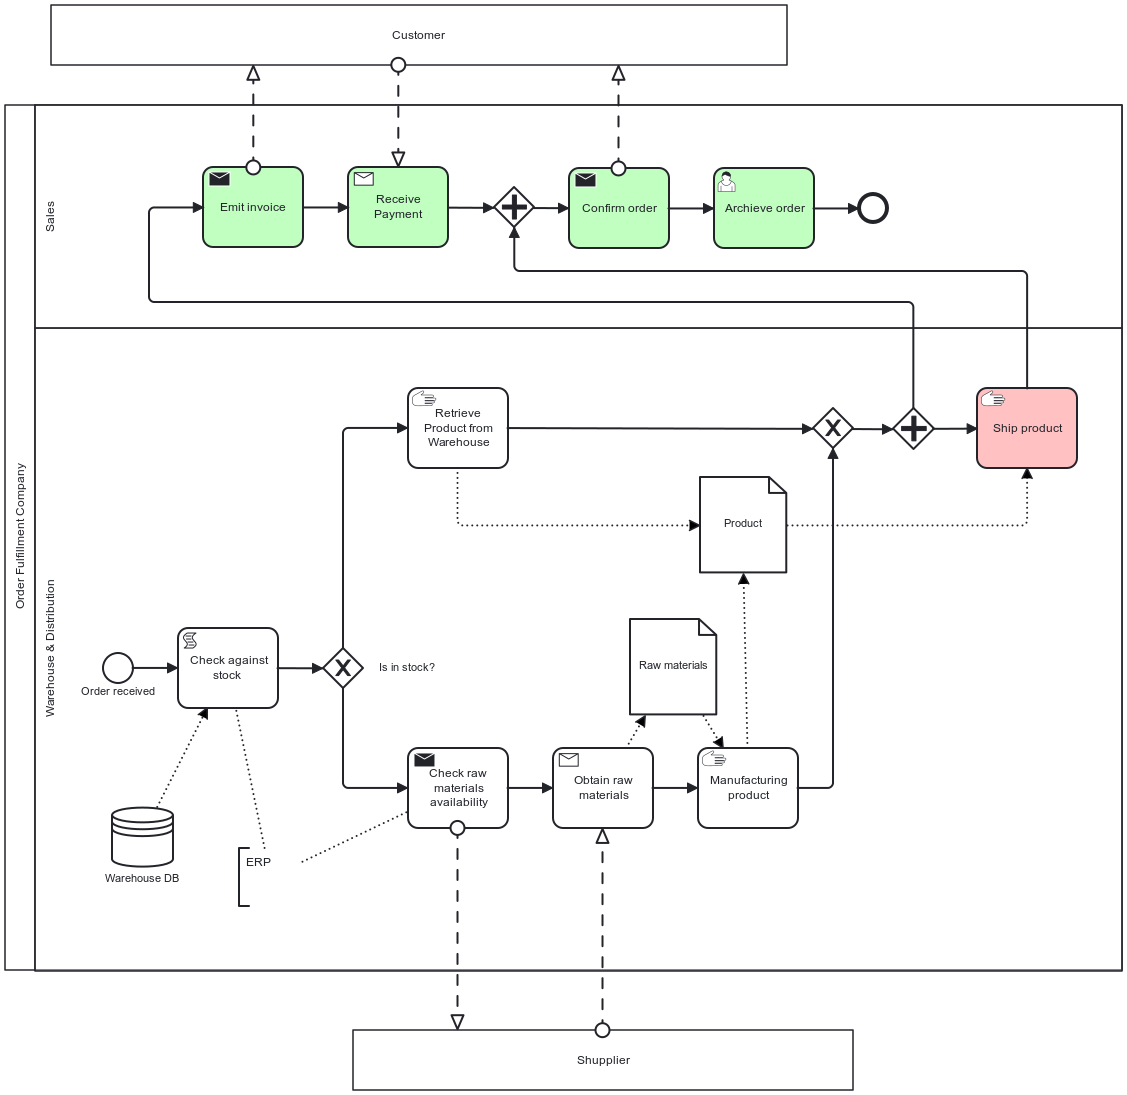
\includegraphics[height=.41\textheight]{images/results/examples/qwen3-235B-run-3-uni-sales-warehouse}
    \caption{Ergebnis des Testfalls \enquote{Sales Warehouse} mit farblich hervorgehobenen Aktivitäten. Grün markierte Aktivitäten sind korrekt als kritisch erkannt, rot markierte stellen \acp{FP} dar.}
    \label{fig:qwen3-fall}
\end{figure}

Das Beispiel verdeutlicht eine grundsätzliche Limitierung der Klassifizierung: Fehlen in einem \ac{BPMN}-Modell explizite Informationen über Verarbeitungsschritte, ist es für das System schwierig, eine eindeutige Klassifikation vorzunehmen.

\subsection*{Marketing-Kampagne}

Im deutschen Testfall \enquote{Marketing-Kampagne}, aus dem Testdatensatz \enquote{Kleine Szenarien}, sind drei Aktivitäten als kritisch gelabelt: \enquote{Leads sammeln}, \enquote{Newsletter versenden} und \enquote{CRM aktualisieren}. \texttt{GPT‑OSS‑20B} identifiziert diese korrekt, markiert aber zusätzlich die Aktivität \enquote{Klickraten auswerten} als kritisch. Die Prozessmodellierung sah vor, dass die Klickdaten komplett anonymisiert werden und daher keine personenbezogenen Daten verarbeitet werden. Da diese Information im \ac{BPMN}-Diagramm jedoch nicht explizit hinterlegt ist, stuft das Modell die Analyse der Klickraten als potenziell personenbezogen ein und führt als Begründung die Nutzung der E‑Mail‑Adresse an. \texttt{Qwen3-235B-A22B-Thinking-2507} und einige weitere Modelle bewerteten diesen Schritt ebenfalls als kritisch, während \texttt{Mistral‑7B‑\linebreak~Instruct‑v0.3} in zwei von fünf Wiederholungen und die Gemma‑Modelle in keiner der Wiederholungen eine kritische Klassifikation vornahmen. Der Prozess inklusive farblich hervorgehobener Aktivitäten ist in Abbildung \ref{fig:gptoss-fall} zu sehen.

Dieses Beispiel zeigt, dass ohne genaue Kontextangaben zur Anonymisierung selbst scheinbar unbedenkliche Auswertungen als datenschutzrelevant erscheinen können. Es unterstreicht, dass die \acp{LLM} im Zweifel eher ein kritisches Label vergeben, um \acp{FN} zu vermeiden, wie es das Hauptziel der Klassifikation aus Abschnitt \ref{sec:qualitatsziele} vorsieht.

\begin{figure}
    \centering
    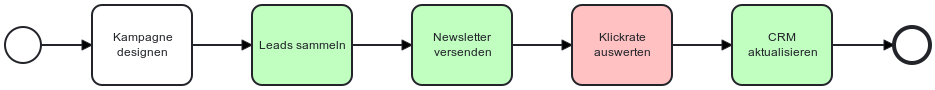
\includegraphics[width=\textwidth]{images/results/examples/oss-20b-run-1-small-marketing}
    \caption{Ergebnis des Testfalls \enquote{Marketing-Kampagne} mit farblich hervorgehobenen Aktivitäten. Die Aktivität \enquote{Klickraten auswerten} wurde als zusätzliches kritisches Element markiert.}
\label{fig:gptoss-fall}
\end{figure}

\subsection*{Karten App - Standort Erfassen}

Im Fall \enquote{Karten-App – Standort Erfassen}, ebenfalls aus dem Testdatensatz \enquote{Kleine Szenarien}, treten zwei Aktivitäten auf: \enquote{Standort erfassen} und \enquote{Route berechnen}. Beide sollten als kritisch gekennzeichnet werden, da im zweiten Schritt der zuvor erfasste Benutzerstandort zur Berechnung der Route verwendet wird. \texttt{Mistral-Large} erkennt jedoch in drei von fünf Läufen nur die erste Aktivität als kritisch und die Aktivität \enquote{Route berechnen} wird trotz der Datenassoziation nicht als kritisch eingestuft. Die Begründung des Modells erklärt zwar, dass \enquote{Standort erfassen} personenbezogene Daten verarbeitet, überträgt diese Argumentation aber nicht auf den unmittelbar folgenden Schritt. Dieses \ac{FN} ist problematisch, da es dem gewünschten hohen Recall entgegensteht und dieser Testfall zeigt, dass selbst mit vorhandenen Datenobjekten manche Modelle Schwierigkeiten haben, Datenflüsse über mehrere Aktivitäten hinweg zu erfassen. Es verdeutlicht auch, dass unterschiedliche Seeds zu unterschiedlichen Klassifikationen führen können. Der Prozess inklusive farblich hervorgehobener Aktivitäten ist in Abbildung \ref{fig:mistral-fall} zu sehen.

\begin{figure}
    \centering
    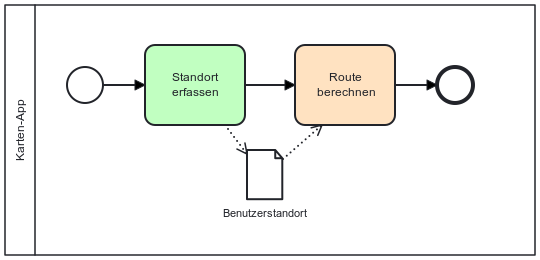
\includegraphics[width=.55\textwidth]{images/results/examples/mistral-large-run-3-small-maps-app}
    \caption{Ergebnis des Testfalls \enquote{Karten-App – Standort Erfassen} mit farblich hervorgehobenen Aktivitäten. Die Aktivität \enquote{Route berechnen} wurde fälschlicherweise nicht als kritisch markiert.}
    \label{fig:mistral-fall}
\end{figure}

Auf Basis der Erkenntnisse dieses gesamten Kapitels werden im folgenden Abschnitt die formulierten Forschungsfragen beantwortet. Dabei wird untersucht welches Modell sich insgesamt am besten für die Identifikation \ac{DSGVO}‑kritischer Aktivitäten eignet.